%%%%%%%%%%%%%%%%%%%%%%%%%%%%%%%%%%%%%%%%%
% Original author:
% Adrien Friggeri (adrien@friggeri.net)
% https://github.com/afriggeri/CV
%
% Modified by:
% Nuno Lourenço (me@nunolourenco.me)
%João Nabais (jlnabais@gmail.com)


\documentclass[]{friggeri-cv} % Add 'print' as an option into the square bracket to remove colors from this template for printing
\usepackage{graphicx}
\usepackage[export]{adjustbox}
\addbibresource{bibliography.bib} % Specify the bibliography file to include publications

\begin{document}
\header{Jo\~ao}{ Casalta Nabais}{Functional Analyst/Software Engineer} % Your name and current job title/field

%----------------------------------------------------------------------------------------
%	SIDEBAR SECTION
%----------------------------------------------------------------------------------------

\begin{aside} % In the aside, each new line forces a line break
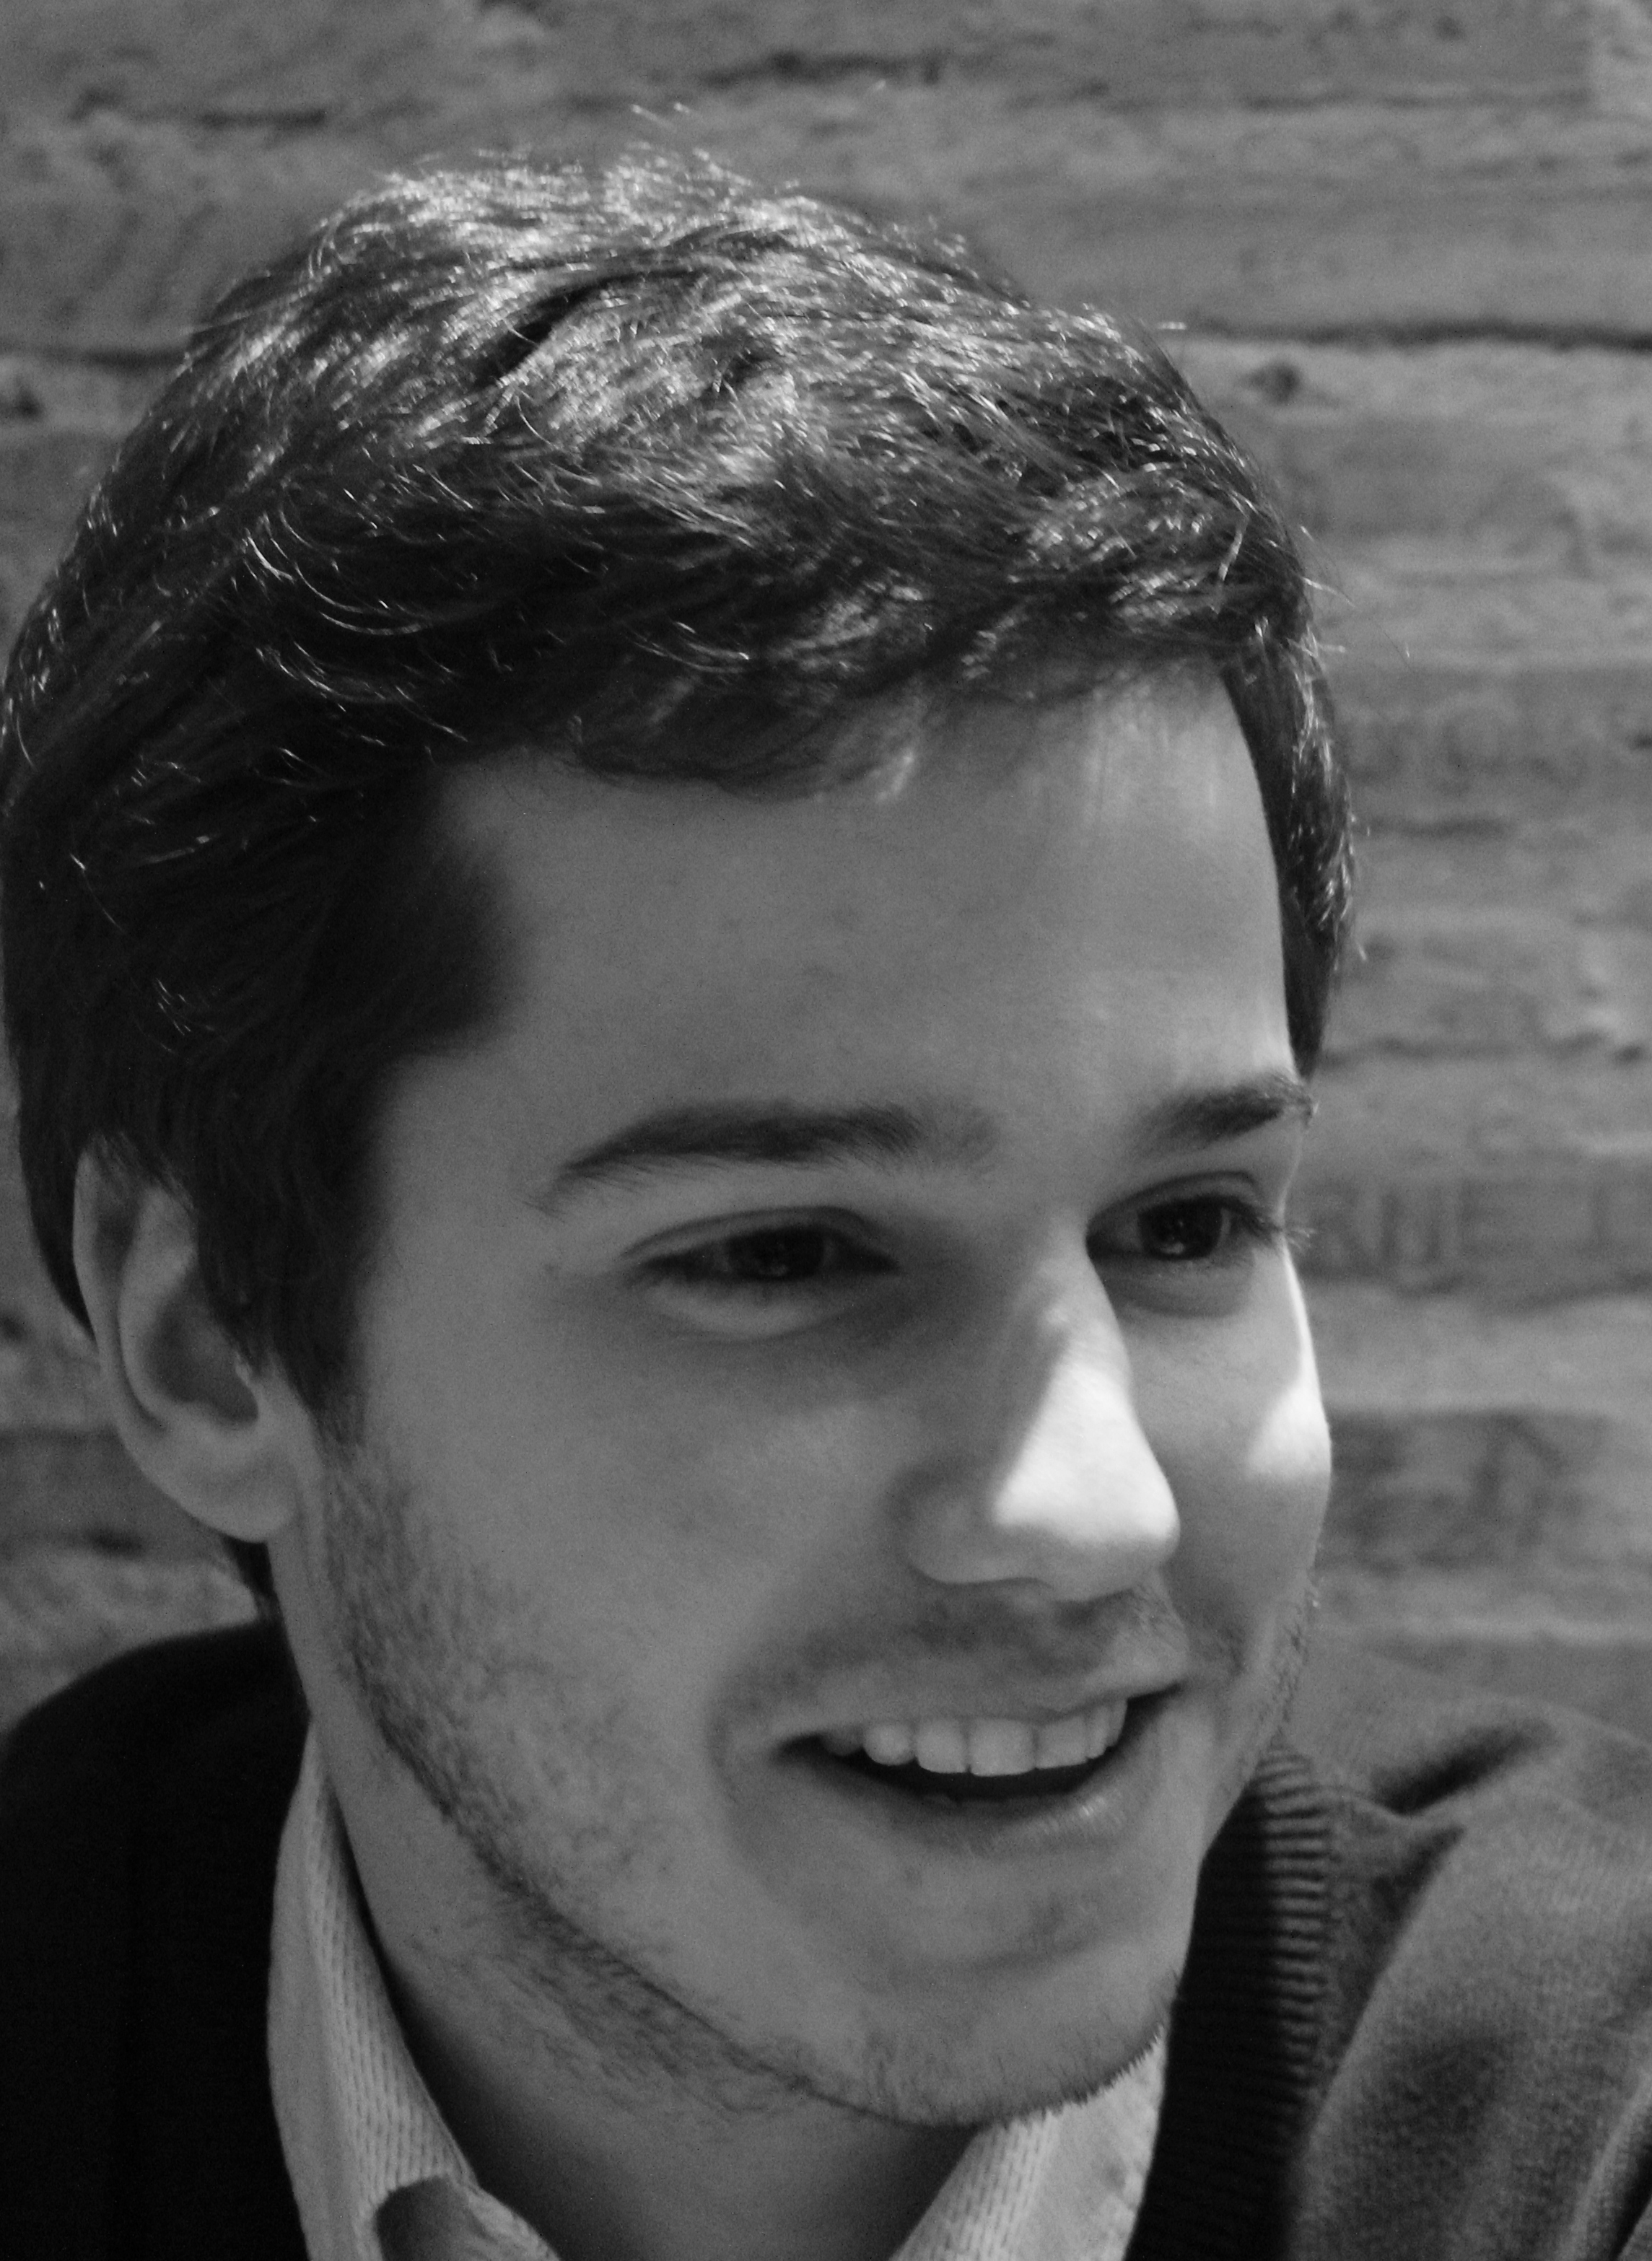
\includegraphics[scale=0.05]{me.png} 
\section{bio}
\includegraphics[scale=0.5, left]{USER.png}
\vspace{-5mm} \textbf{Name}: João Luís Gomes Marques Casalta Nabais
\includegraphics[scale=0.5, left]{calendar.png}
\vspace{-5mm} \textbf{Birth}: August 7, 1987
\includegraphics[scale=0.5, left]{flag.png}
\vspace{-5mm} \textbf{Citizenship}: Portuguese
\includegraphics[scale=0.5, left]{location.png} 
\vspace{-5mm} \textbf{Lives in}: Lisboa, Portugal
\section{contacts}
\includegraphics[scale=0.5, left]{phone.png} 
\vspace{-5mm} +351 918865622
\includegraphics[scale=0.5, left]{envelope.png}
\vspace{-5mm} \href{mailto:jlnabais@gmail.com}{jlnabais@gmail.com}
\includegraphics[scale=0.5, left]{linkedin.png} 
\vspace{-5mm} \href{http://www.linkedin.com/in/jlnabais}{jlnabais}
\section{languages}
\includegraphics[scale=0.5, left]{globe.png}
\vspace{-5mm} Portuguese native
English fluent
Spanish elementary
\section{technologies}
\includegraphics[scale=0.5, left]{cogs.png}
\vspace{-5mm}  Python, C\#, javascript
Django, JQuery, Bootstrap
RDF, OWL
\section{interests}
\includegraphics[scale=0.5, left]{like.png}
\vspace{-5mm} ITSM, ITIL, BPMN \\ Semantic Web
\end{aside}



%----------------------------------------------------------------------------------------
%	EDUCATION SECTION
%----------------------------------------------------------------------------------------


\section{Education}

\begin{entrylist}
%------------------------------------------------
\entrymasters
{2011--2013}
{Masters {\normalfont in Informatics Engineering}}
{University of Coimbra, Portugal}
{\emph{Thesis: InTeligent - Interoperable Telecommunications ITIL-compliant Services Management System} \\ This thesis proposed the development of potentially standardizable and reusable ITIL components interfaces (in partnership with PT Comunicações, SA/DTS - Sapo Technology Department), as well as the development of a Service Portfolio Management System, based on Semantic Web Technologies.}
{\textbf{University Advisors:} Dr. Alexandre Pinto and Dr. Jorge Cardoso}
{\textbf{Industry Advisors:} António Cruz}
{\textbf{Thesis Grade:} 19/20}
%------------------------------------------------
\entrybachelor
{2006--2011}
{Bachelor {\normalfont in Informatics Engineering}}
{University of Coimbra, Portugal}
%------------------------------------------------
\end{entrylist}

%----------------------------------------------------------------------------------------
%	WORK EXPERIENCE SECTION
%----------------------------------------------------------------------------------------
\section{Experience}

\begin{entrylist}
%------------------------------------------------
\entry
{2013--\emph{Present}}
{Functional Analyst and Software Engineer}
{Portugal Telecom}
{\emph{Functional Analyst and Software Engineer (SAPO Service Delivery Broker)}\\
Analysis of ITIL processes (from Service Operation, Service Transition and Service Design).\\
Development (C\#/.NET) of a support service, part of by ITSM Web Application.}
%------------------------------------------------
\entry
{2012-2013}
{Functional Analyst}
{SAPO Labs (Coimbra)}
{\emph{Functional Analyst}\\
Development of a set of interfaces for Problem and Incident Management (ITIL Processes).}
%------------------------------------------------
\entry
{2012-2013}
{Researcher}
{Centre for Informatics and Systems of the University of Coimbra}
{\emph{Researcher at Information Systems Group}\\
Development of a Service Portfolio Management System re-using semantic web technologies and developing an ontology for ITSM Services.}
%------------------------------------------------

\end{entrylist}

%----------------------------------------------------------------------------------------
%	AWARDS SECTION
%----------------------------------------------------------------------------------------

\section{Honors \& Awards}

\begin{entrylist}
%------------------------------------------------
\entry
{2012-2013}
{MSc Scholarship}
{SAPO Labs}
{InTeligent Project}
%------------------------------------------------
\end{entrylist}

%----------------------------------------------------------------------------------------
%	PUBLICATIONS SECTION
%----------------------------------------------------------------------------------------

\section{Publications}

\begin{refsection} % This is a custom heading for those references marked as "inproceedings" but not containing "keyword=france"
\nocite{*}
\printbibliography[sorting=chronological, type=inproceedings, title={international peer-reviewed conferences/proceedings}, notkeyword={france}, heading=subbibliography]
\end{refsection}

%----------------------------------------------------------------------------------------

\vfill\eject

%----------------------------------------------------------------------------------------
%	ORGANIZATIONAL SKILLS SECTION
%----------------------------------------------------------------------------------------

\section{Organizational Skills}

\begin{entrylist}
%------------------------------------------------
\entry
{2012}
{Ubiquitous Systems Workshop}
{University of Coimbra}
{\emph{Co-organizer of the ubiquitous systems course workshop}}
%------------------------------------------------
\entry
{2009}
{Electoral Commission}
{University of Coimbra}
{\emph{Delegate of the electoral commission president for the statutory revision assembly of the academic association of Coimbra}}
%------------------------------------------------
\entry
{2009}
{Electoral Commission}
{University of Coimbra}
{\emph{Member of the electoral commission for the assembly and pedagogic council of Coimbra university's faculty of sciences and technology}}
%------------------------------------------------
\entry
{2008}
{Electoral Commission}
{University of Coimbra}
{\emph{President of the electoral commission for the student body of the Faculty of Sciences and Technology of the University of Coimbra}}
%------------------------------------------------
\entry
{2008}
{Weekid Event}
{University of Coimbra}
{\emph{Co-organizer of a public event for child obesity awareness}}
%------------------------------------------------
\end{entrylist}

\end{document}